\begin{figure}[h!]
%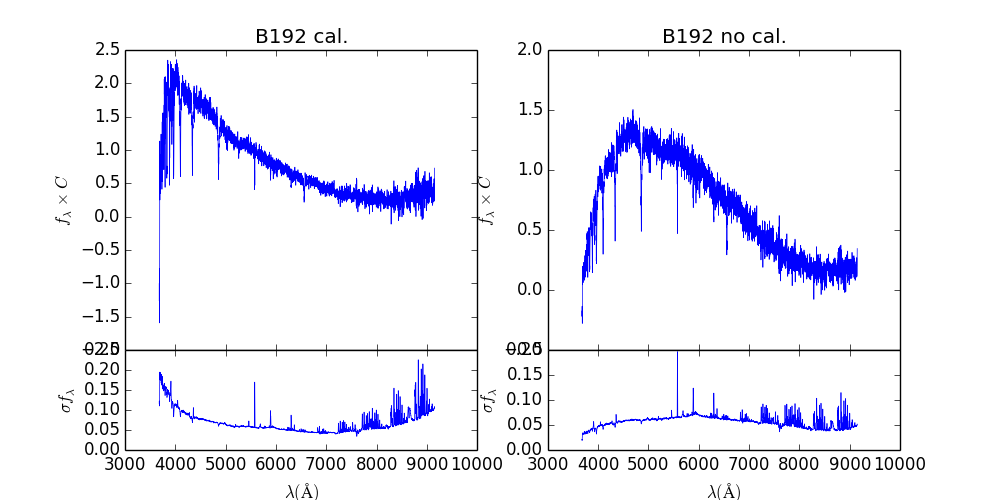
\includegraphics[width = 0.5 \textwidth]{figures/dfig_b192-g242_020.png}
\caption{The calibrated spectrum for \excluster, along with the
uncertainties (bottom panel).The right panel shows the
spectrophotometric calibration vector determined by
\citet{schiavon05}. \label{fig:ggc_data}}
\end{figure}

\begin{figure}[h!]
%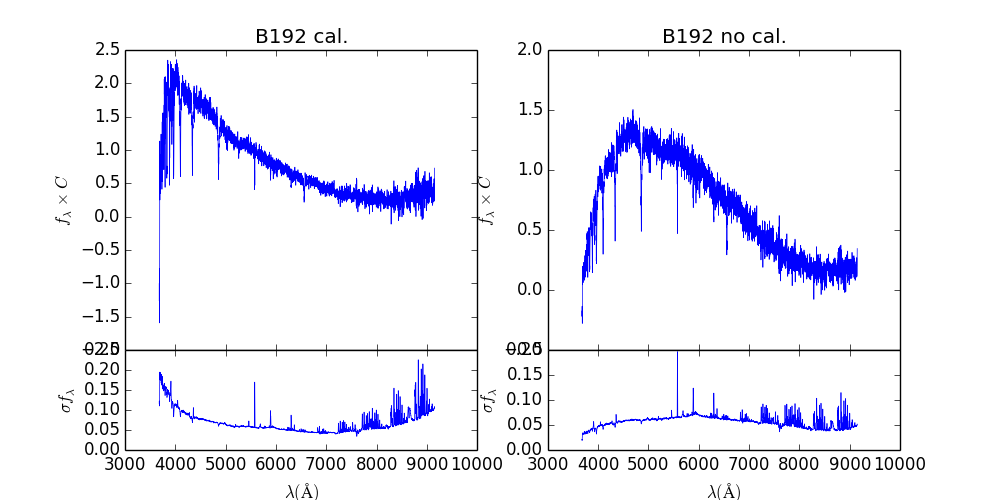
\includegraphics[width = 0.5 \textwidth]{figures/dfig_b192-g242_020.png}
\caption{A mock spectrum for a star cluster with $10^5 M_\odot$ total
  stellar mass, an age of  9 Gyr, solar
  metallicity, and $A_V=0.5$ mag. \label{fig:mock_data}}
\end{figure}


\begin{figure*}[h!]
%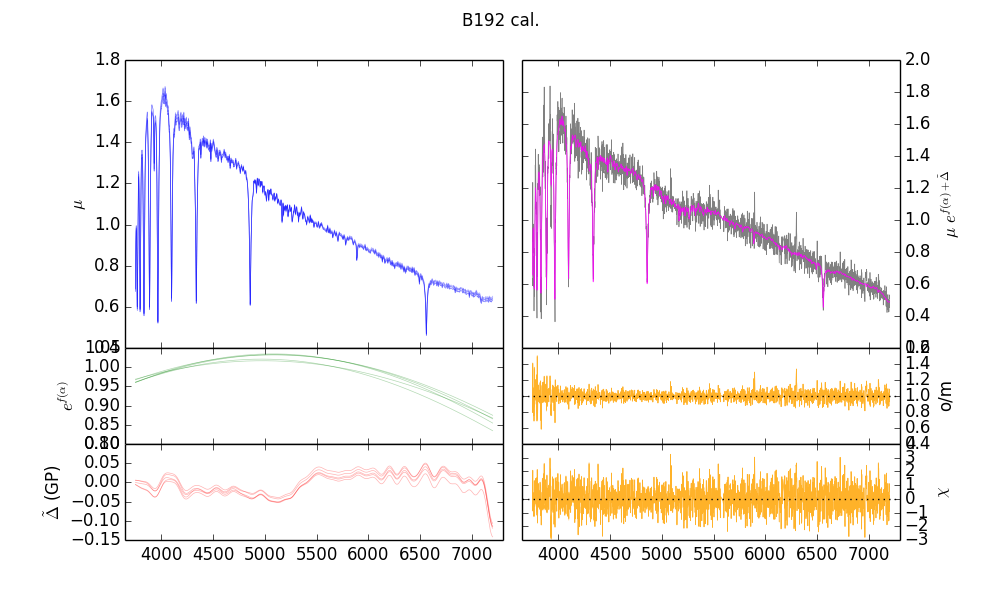
\includegraphics[width=\textwidth]{figures/sfig_b192-g242_225_cal.png}
\caption{Results of inference from a mock spectrum and a single photometric data point where the spectrophotometric calibration is assumed to be perfectly known.
Top Left: The mock observed spectrum ({\it black}) is shown as well as
YY model spectra constructed from draws from the posterior PDFs of the
model parameters, including calibration parameters {\it green}.
Bottom Left: In this case the true calibration vector ({\it black}) is a constant.
Posterior samples of the inferred calibration vector ({\it green}) include both
the polynomial and the Gaussian Process mean prediction (Equation
\ref{eq:calibration}).
Top Right: Samples of the posterior prediction for the
\emph{intrinsic} spectrum ({\it green}) as well as for the photometry
({\it magenta}).  The true mock photometry is also shown ({\it
black}).
Bottom Right: Marginalized posterior PDFs for several of the physical
parameters of interest.  The input mock parameters are shown as
vertical lines.
\label{fig:speconly_ideal}}
\end{figure*}


\begin{figure*}[h!]
%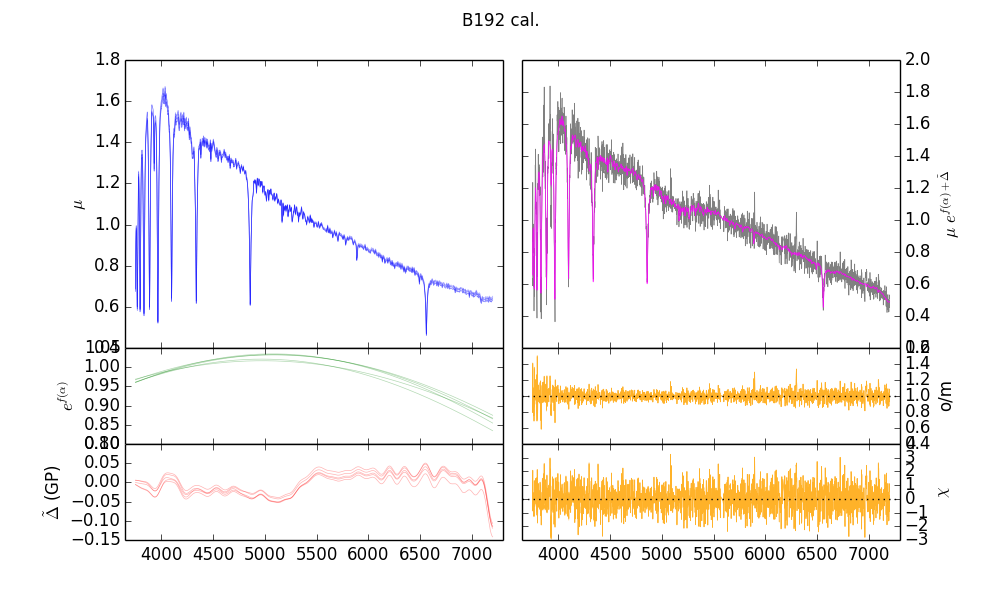
\includegraphics[width=\textwidth]{figures/sfig_b192-g242_225_cal.png}
\caption{Results of inference from a \emph{perfectly calibrated} mock
  spectrum and a single photometric data point.
Top Left: The mock observed spectrum ({\it black}) is shown as well as
YY model spectra constructed from draws from the posterior PDFs of the
model parameters, including calibration parameters {\it green}.
Bottom Left: In this case the true calibration vector ({\it black}) is a constant.
Posterior samples of the inferred calibration vector ({\it green}) include both
the polynomial and the Gaussian Process mean prediction (Equation
\ref{eq:calibration}).
Top Right: Samples of the posterior prediction for the
\emph{intrinsic} spectrum ({\it green}) as well as for the photometry
({\it magenta}).  The true mock photometry is also shown ({\it
black}).
Bottom Right: Marginalized posterior PDFs for several of the physical
parameters of interest.  The input mock parameters are shown as
vertical lines.
\label{fig:speconly_calibrated}}
\end{figure*}

\begin{figure*}[h!]
%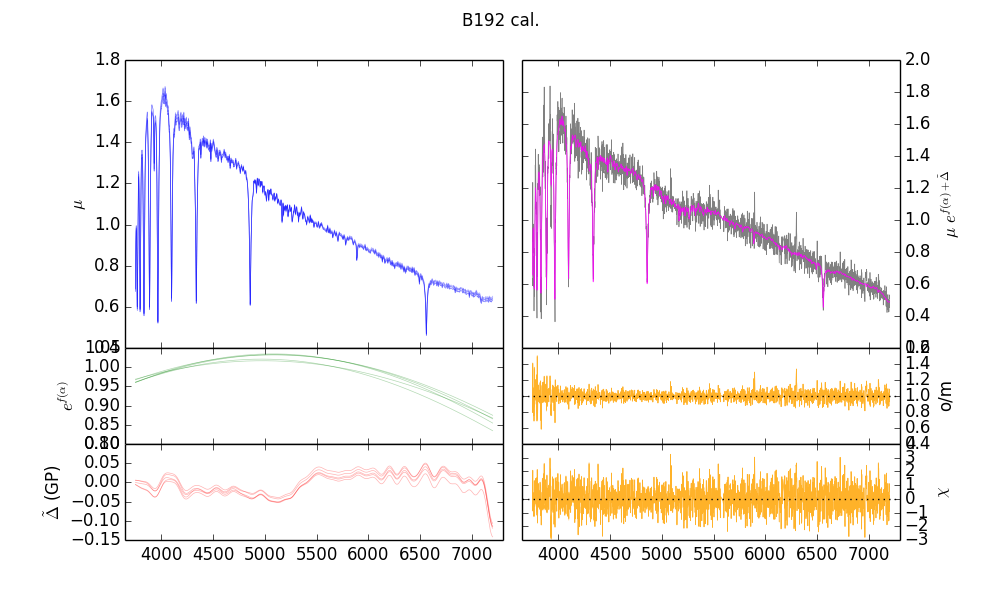
\includegraphics[width=\textwidth]{figures/sfig_b192-g242_225_cal.png}
\caption{Results of inference from an \emph{uncalibrated} mock
  spectrum and a single photometric data point.
Top Left: The observed spectrum. The mock observed spectrum ({\it
black}) is shown as well as YY model spectra constructed from draws
from the posterior PDFs of the model parameters, including calibration
parameters {\it green}.
Bottom Left: The calibration vector. The true calibration vector ({\it
black}) that was used to construct the mock spectrum is compared to
posterior samples of the inferred calibration vector ({\it green})
which include both the polynomial and the Gaussian Process mean
prediction (Equation
\ref{eq:calibration}).
Top Right: The intrinsic spectrum. Samples of the posterior prediction
for the \emph{intrinsic} spectrum ({\it green}) as well as for the
photometry ({\it magenta}).  The true mock photometry is also shown
({\it black}).
Bottom Right: Marginalized posterior PDFs for several of the physical
parameters of interest.  The input mock parameters are shown as
vertical lines.
\label{fig:speconly_calibrated}}
\end{figure*}

\begin{figure*}[h!]
%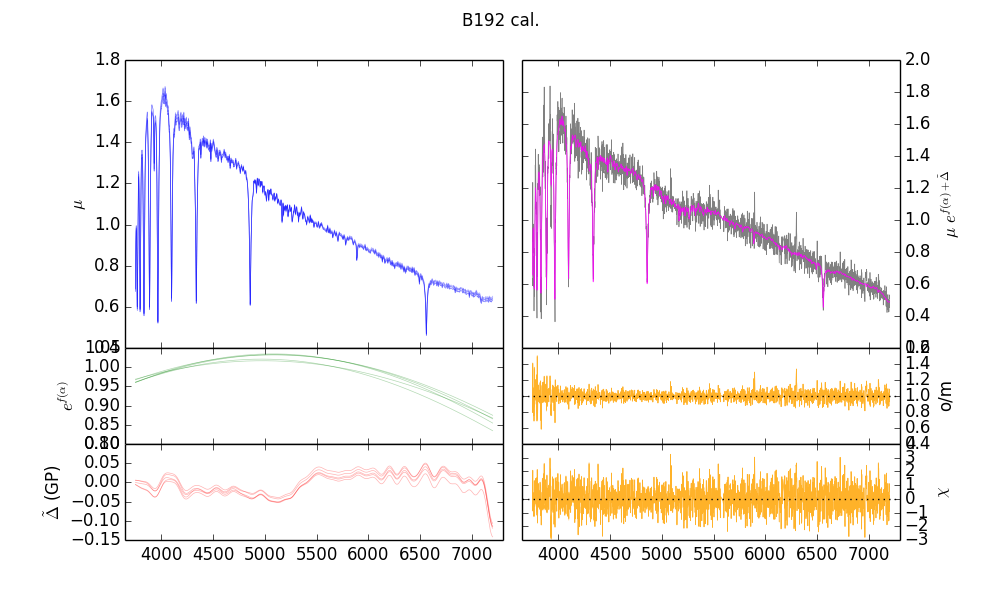
\includegraphics[width=\textwidth]{figures/sfig_b192-g242_225_cal.png}
\caption{Results of inference from the photometry only.
Top: The intrinsic spectrum. Samples of the posterior prediction
for the \emph{intrinsic} spectrum ({\it green}) as well as for the
photometry ({\it magenta}).  The true mock photometry is also shown
({\it black}).
Right: Marginalized posterior PDFs for several of the physical
parameters of interest.  The input mock parameters are shown as
vertical lines.
\label{fig:speconly_calibrated}}
\end{figure*}

\begin{figure*}[h!]
%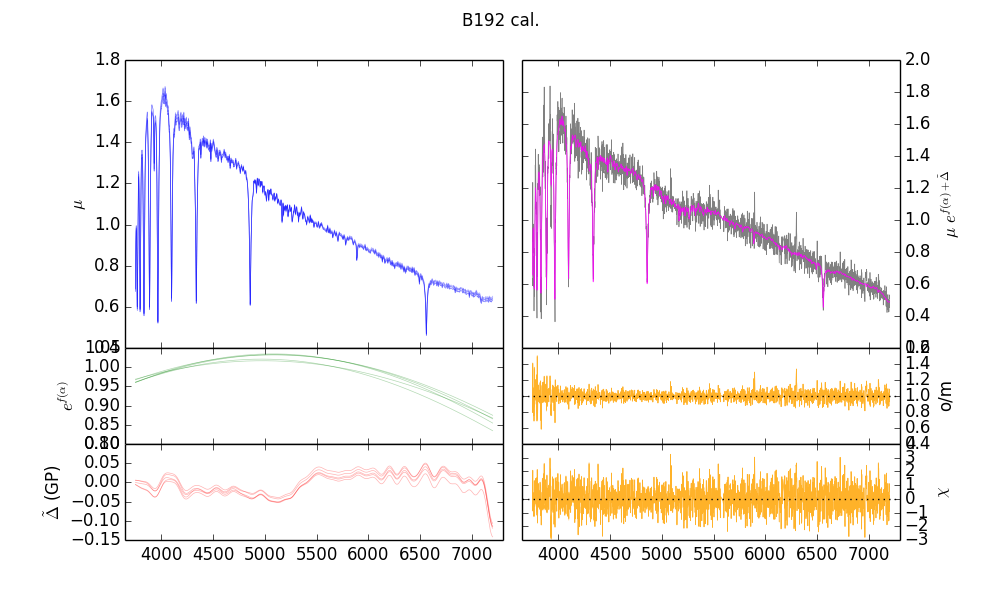
\includegraphics[width=\textwidth]{figures/sfig_b192-g242_225_cal.png}
\caption{Results of inference from the combination of mock 
Top Left: The observed spectrum. The mock observed spectrum ({\it
black}) is shown as well as YY model spectra constructed from draws
from the posterior PDFs of the model parameters, including calibration
parameters {\it green}.
Bottom Left: The calibration vector. The true calibration vector ({\it
black}) that was used to construct the mock spectrum is compared to
posterior samples of the inferred calibration vector ({\it green})
which include both the polynomial and the Gaussian Process mean
prediction (Equation
\ref{eq:calibration}).
Top Right: The intrinsic spectrum. Samples of the posterior prediction
for the \emph{intrinsic} spectrum ({\it green}) as well as for the
photometry ({\it magenta}).  The true mock photometry is also shown
({\it black}).
Bottom Right: Marginalized posterior PDFs for several of the physical
parameters of interest.  The input mock parameters are shown as
vertical lines.
\label{fig:speconly_calibrated}}
\end{figure*}
